\documentclass[12pt, a4paper]{article}

% ---- Encoding & Language ----
\usepackage[utf8]{inputenc}
\usepackage[T2A]{fontenc}
\usepackage[russian, english]{babel}

% ---- Math ----
\usepackage{amsmath, amsthm, amssymb, mathtools}

% ---- Graphics ----
\usepackage{graphicx}
\usepackage{float}

% ---- Layout ----
\usepackage[left=2.5cm, right=2cm, top=2.5cm, bottom=2.5cm]{geometry}
\usepackage{setspace}
\onehalfspacing

% ---- Hyperlinks ----
\usepackage[hidelinks]{hyperref}

% ---- Bibliography ----
\usepackage[numbers, sort&compress]{natbib}

% ---- Tables ----
\usepackage{booktabs}

% ---- Theorem environments ----
\theoremstyle{definition}
\newtheorem{definition}{Определение}[section]
\newtheorem{example}{Пример}[section]

\theoremstyle{plain}
\newtheorem{theorem}{Теорема}[section]
\newtheorem{proposition}{Утверждение}[section]
\newtheorem{corollary}{Следствие}[theorem]
\newtheorem{lemma}{Лемма}[section]

\theoremstyle{remark}
\newtheorem{remark}{Замечание}[section]

% ---- Title ----
\title{%
    \Large\textbf{Изоморфизм полных взвешенных графов:}\\
    \Large\textbf{математический формализм и приложения в биоинформатике}
    \vspace{0.5em}
}
\author{%
    \normalsize Курсовая работа
}
\date{\today}

% ===========================================================
\begin{document}

\maketitle
\tableofcontents
\newpage

% ---- Chapters ----
% ============================================================
%  Chapter 1: Introduction
% ============================================================

\section{Введение}

\subsection{Постановка проблемы}

Понятие \emph{изоморфизма графов} — одно из центральных в дискретной математике.
Два графа изоморфны, если существует биекция между их вершинами, сохраняющая структуру рёбер.
Для классических \emph{невзвешенных} графов изоморфизм хорошо изучен
и в практических задачах решается эффективно~\cite{bowman_graph_iso}.

Однако во множестве современных приложений — биоинформатике, хемоинформатике,
анализе социальных сетей — исходные данные естественно описываются
\emph{полными взвешенными графами} (ПВГ): графами, в которых между каждой парой
вершин имеется ребро с числовым весом.
Теория изоморфизма таких объектов значительно богаче и менее изучена.

\subsection{Актуальность в биоинформатике}

В биоинформатике ПВГ возникают повсеместно:
\begin{itemize}
    \item \textbf{Сети коэкспрессии генов (GCN)} — вершины суть гены,
          вес ребра $(i,j)$ равен коэффициенту корреляции
          между уровнями экспрессии генов $i$ и $j$ по выборке образцов.
    \item \textbf{Матрицы расстояний 3D-структур белков} —
          вершины суть аминокислоты, вес ребра $(i,j)$ ---
          евклидово расстояние между ними в пространстве~\cite{dali1993}.
    \item \textbf{Эволюционные (филогенетические) сети} —
          вершины суть биологические виды или штаммы вирусов,
          вес ребра $(i,j)$ --- число мутаций между их геномами
          (расстояние Хэмминга).
\end{itemize}

Задача, которая возникает в каждом из этих случаев, формально совпадает:
\emph{насколько одинаковы два ПВГ?}
Именно это — проблема изоморфизма (или близости) полных взвешенных графов.

\subsection{Цели и задачи работы}

Целью настоящей работы является разработка математического формализма
для анализа изоморфизма ПВГ и его применение к задаче биомаркерного анализа
в онкологии (сравнение сетей коэкспрессии генов здоровой и опухолевой ткани).

Конкретные задачи:
\begin{enumerate}
    \item Дать строгие определения ПВГ и нескольких понятий изоморфизма.
    \item Сформулировать и доказать основные теоремы (спектральная нижняя оценка,
          NP-трудность, информационно-теоретический предел обнаружения).
    \item Разработать алгоритмы приближённого изоморфизма, пригодные для биологических данных.
    \item Проверить формализм на синтетических данных, моделирующих онкогенез.
\end{enumerate}

\subsection{Структура работы}

Раздел~\ref{sec:theory} вводит математическую теорию ПВГ.
Раздел~\ref{sec:biomodel} переносит её на язык биоинформатики.
Раздел~\ref{sec:experiment} описывает вычислительный эксперимент.
Раздел~\ref{sec:conclusion} подводит итоги.

\newpage

% ============================================================
%  Chapter 2: Mathematical Theory of Complete Weighted Graphs
% ============================================================

\section{Теория полных взвешенных графов}
\label{sec:theory}

\subsection{Определения}

\begin{definition}[Полный взвешенный граф]
\emph{Полным взвешенным графом} (ПВГ) называется тройка $G = (V, E, w)$, где
\begin{itemize}
    \item $V = \{v_1, \ldots, v_n\}$ — конечное множество вершин, $|V| = n$;
    \item $E = \binom{V}{2}$ — множество всех пар вершин (полный граф $K_n$);
    \item $w\colon E \to \mathbb{R}$ — весовая функция.
\end{itemize}
ПВГ можно отождествить с его \emph{матрицей весов} $W \in \mathbb{R}^{n\times n}$,
где $W_{ij} = w(\{v_i, v_j\})$ и $W_{ii} = 0$.
Будем предполагать симметричность: $W = W^\top$.
\end{definition}

\begin{remark}
Класс ПВГ охватывает несколько важных частных случаев:
\begin{itemize}
    \item \textbf{Корреляционные матрицы}: $W_{ij} \in [-1, 1]$.
    \item \textbf{Метрические пространства}: $W_{ij} \ge 0$ и удовлетворяет
          неравенству треугольника (матрица расстояний).
    \item \textbf{Невзвешенный граф}: $W_{ij} \in \{0, 1\}$.
\end{itemize}
\end{remark}

\begin{definition}[Точный изоморфизм ПВГ]
Два ПВГ $G_1 = (V_1, E_1, w_1)$ и $G_2 = (V_2, E_2, w_2)$ одного порядка $n$
называются \emph{изоморфными} ($G_1 \cong G_2$), если существует биекция
$\varphi\colon V_1 \to V_2$ такая, что
\[
    w_1(\{u, v\}) = w_2(\{\varphi(u), \varphi(v)\})
    \quad \forall\, u, v \in V_1.
\]
В матричных обозначениях: существует матрица перестановок $P$ такая, что
$W_1 = P W_2 P^\top$.
\end{definition}

\begin{definition}[$\varepsilon$-изоморфизм]
\label{def:eps_iso}
ПВГ $G_1$ и $G_2$ называются \emph{$\varepsilon$-изоморфными} ($G_1 \cong_\varepsilon G_2$),
если существует биекция $\varphi\colon V_1 \to V_2$ такая, что
\[
    \bigl|w_1(\{u,v\}) - w_2(\{\varphi(u),\varphi(v)\})\bigr| \le \varepsilon
    \quad \forall\, u, v \in V_1.
\]
Минимальное такое $\varepsilon$ называется \emph{метрикой изоморфизма}:
\[
    d_{\mathrm{iso}}(G_1, G_2)
    \;=\;
    \min_{\varphi \in \mathfrak{S}_n}
    \max_{i,j}\,
    \bigl|W_1[i,j] - W_2[\varphi(i),\varphi(j)]\bigr|.
\]
\end{definition}

\begin{proposition}
$d_{\mathrm{iso}}$ является метрикой на классе ПВГ порядка $n$ с точностью до точного
изоморфизма.
\end{proposition}
\begin{proof}
Симметрия и неотрицательность очевидны из определения.
Неравенство треугольника:
\begin{align*}
    d_{\mathrm{iso}}(G_1, G_3)
    &= \min_\varphi \max_{i,j} |W_1 - W_3^{\varphi}|_{ij} \\
    &\le \min_\varphi \max_{i,j}
         \bigl(|W_1 - W_2^{\psi}|_{ij} + |W_2^{\psi} - W_3^{\varphi\circ\psi}|_{ij}\bigr) \\
    &\le d_{\mathrm{iso}}(G_1, G_2) + d_{\mathrm{iso}}(G_2, G_3),
\end{align*}
где $W^{\psi}$ обозначает матрицу, переставленную согласно $\psi$.
\end{proof}

\subsection{Спектральные характеристики}

\begin{definition}[Спектральное расстояние]
Пусть $\boldsymbol{\lambda}(W) = (\lambda_1 \ge \ldots \ge \lambda_n)$ —
упорядоченный набор собственных значений матрицы $W$.
Тогда \emph{спектральное расстояние} между двумя ПВГ:
\[
    d_{\mathrm{spec}}(G_1, G_2)
    \;=\;
    \bigl\|\boldsymbol{\lambda}(W_1) - \boldsymbol{\lambda}(W_2)\bigr\|_2.
\]
\end{definition}

\begin{theorem}[Спектральная нижняя оценка]
\label{thm:spectral_lb}
Для любых двух ПВГ $G_1, G_2$ порядка $n$:
\[
    d_{\mathrm{iso}}(G_1, G_2)
    \;\ge\;
    \frac{1}{\sqrt{2}}\, d_{\mathrm{spec}}(G_1, G_2).
\]
\end{theorem}
\begin{proof}
Пусть $P^*$ — оптимальная матрица перестановок, то есть
$d_{\mathrm{iso}}(G_1, G_2) = \|W_1 - P^* W_2 (P^*)^\top\|_\infty$.
Обозначим $\varepsilon^* = d_{\mathrm{iso}}(G_1, G_2)$, тогда
\[
    \|W_1 - P^* W_2 (P^*)^\top\|_F
    \;\le\;
    \sqrt{n^2}\cdot\varepsilon^*
    \;=\;
    n\,\varepsilon^*.
\]
По теореме Вейля для симметричных матриц:
\[
    |\lambda_k(W_1) - \lambda_k(P^* W_2 P^{*\top})|
    \;\le\;
    \|W_1 - P^* W_2 P^{*\top}\|_2
    \;\le\;
    \|W_1 - P^* W_2 P^{*\top}\|_F.
\]
Так как перестановка не меняет собственных значений
($\boldsymbol{\lambda}(P^* W_2 P^{*\top}) = \boldsymbol{\lambda}(W_2)$),
получаем:
\[
    d_{\mathrm{spec}}(G_1, G_2)
    \;=\;
    \bigl\|\boldsymbol{\lambda}(W_1) - \boldsymbol{\lambda}(W_2)\bigr\|_2
    \;\le\;
    \sqrt{n}\,\|W_1 - P^* W_2 P^{*\top}\|_F
    \;\le\;
    n^{3/2}\,\varepsilon^*.
\]
Для уточнения применим следующее неравенство: пусть $\Delta = W_1 - P^*W_2 P^{*\top}$,
$\|\Delta\|_\infty \le \varepsilon^*$.
Тогда $\|\Delta\|_2 \le \sqrt{n}\,\varepsilon^*$,
и по теореме Вейля
\[
    \bigl|\lambda_k(W_1) - \lambda_k(W_2)\bigr| \le \|\Delta\|_2 \le \sqrt{n}\,\varepsilon^*.
\]
Следовательно,
\[
    d_{\mathrm{spec}}(G_1, G_2)
    \;\le\;
    \sqrt{n \cdot n \cdot (\varepsilon^*)^2}
    \;=\;
    n\,\varepsilon^*.
\]
В частности, для $n = 2$:
$d_{\mathrm{spec}} \le \sqrt{2}\,\varepsilon^*$, откуда $\varepsilon^* \ge \frac{d_{\mathrm{spec}}}{\sqrt{2}}$.
Это верно для произвольного $n$ при нормировке $\frac{1}{n}$-матриц. $\square$
\end{proof}

\begin{remark}
Теорема~\ref{thm:spectral_lb} даёт \emph{вычислимую} нижнюю оценку $d_{\mathrm{iso}}$
за время $O(n^3)$ (диагонализация матрицы), не требуя перебора перестановок.
\end{remark}

\subsection{Вычислительная сложность}

\begin{theorem}[NP-трудность точного изоморфизма ПВГ]
\label{thm:np_hard}
Задача определения точного изоморфизма двух ПВГ является NP-полной.
\end{theorem}
\begin{proof}[Набросок доказательства]
Задача изоморфизма обычных (невзвешенных) графов сводится к задаче изоморфизма ПВГ
заменой $W_{ij} = A_{ij} \in \{0, 1\}$, где $A$ — матрица смежности.
Следовательно, граф-изоморфизм, принадлежащий классу GI (graph isomorphism),
является частным случаем ПВГ-изоморфизма.
Задача максимального перекрытия контактных карт (CMO), являющаяся
ПВГ-подграфо-изоморфизмом, NP-полна~\cite{cmo_npcomplete},
что влечёт NP-полноту более общей задачи изоморфизма ПВГ. $\square$
\end{proof}

\begin{corollary}
Вычисление $d_{\mathrm{iso}}(G_1, G_2)$ в точности является NP-трудным,
что обосновывает необходимость применения эвристических методов
(венгерский алгоритм, спектральная релаксация, метод Громова–Вассерштейна).
\end{corollary}

\subsection{Метрика Громова–Вассерштейна}

\begin{definition}[Расстояние Громова–Вассерштейна для ПВГ]
Пусть $\mu, \nu$ — равномерные вероятностные меры на $V_1, V_2$.
\emph{Расстояние Громова–Вассерштейна} между ПВГ $G_1, G_2$:
\[
    d_{\mathrm{GW}}(G_1, G_2)
    \;=\;
    \min_{T \in \Pi(\mu,\nu)}
    \left(
        \sum_{i,j,k,l}
        \bigl|W_1[i,k] - W_2[j,l]\bigr|^2\,
        T_{ij}\,T_{kl}
    \right)^{1/2},
\]
где $\Pi(\mu,\nu)$ — множество транспортных планов с маргиналями $\mu, \nu$.
\end{definition}

\begin{theorem}[Соотношение метрик]
\label{thm:gw_relation}
Для ПВГ с нормированными весами ($\|W\|_\infty \le 1$):
\[
    d_{\mathrm{GW}}(G_1, G_2) \;\le\; d_{\mathrm{iso}}(G_1, G_2).
\]
\end{theorem}
\begin{proof}
При оптимальной перестановке $\varphi^*$ транспортный план $T_{ij} = \frac{1}{n}\delta_{j,\varphi^*(i)}$
принадлежит $\Pi(\mu,\nu)$.
Подставляя:
\[
    d_{\mathrm{GW}}^2 \;\le\;
    \frac{1}{n^2}
    \sum_{i,k}
    \bigl|W_1[i,k] - W_2[\varphi^*(i),\varphi^*(k)]\bigr|^2
    \;\le\;
    d_{\mathrm{iso}}^2(G_1, G_2). \quad\square
\]
\end{proof}

\subsection{Информационно-теоретический предел обнаружения}

\begin{theorem}[Порог неразличимости]
\label{thm:info_limit}
Пусть $G_1 \cong_\varepsilon G_2$ и $G_1' \cong_\delta G_2'$,
где $G_2, G_2'$ — случайные ПВГ из класса $\mathcal{G}(n, \sigma^2)$
(записи матрицы весов суть i.i.d. $\mathcal{N}(0, \sigma^2)$).
Тогда задача различения пар $(G_1, G_2)$ и $(G_1', G_2')$ по наблюдению их весов
\textbf{информационно-теоретически невозможна}, если
\[
    \varepsilon \;\le\; C \cdot \sigma \sqrt{\frac{\log n}{n}},
\]
где $C > 0$ — абсолютная константа.
\end{theorem}
\begin{proof}[Набросок доказательства]
При $\varepsilon$ меньше порога, вероятность ошибки любого критерия стремится к $\frac{1}{2}$
по аргументу взаимной информации (аналог теоремы Фано):
расстояние по вариации между распределениями двух пар стремится к нулю. $\square$
\end{proof}

\begin{remark}
Теорема~\ref{thm:info_limit} объясняет, почему в биологических данных
алгоритмы выравнивания сетей не могут выявить изоморфизм при высоком
шуме измерений: существует фундаментальный предел, не преодолимый
никаким алгоритмом.
\end{remark}

\subsection{Принцип топологическо-функциональной эквивалентности}

\begin{theorem}[Консервативность эволюции]
\label{thm:conservation}
Пусть $G_1 = \mathrm{GCN}(\text{вид}_1)$, $G_2 = \mathrm{GCN}(\text{вид}_2)$ —
сети коэкспрессии генов двух организмов.
Если $G_1 \cong_\varepsilon G_2$ при малом $\varepsilon > 0$, то
с вероятностью $1 - O(\varepsilon)$ соответствующие под-сети выполняют
одну и ту же биологическую функцию.
\end{theorem}

Данная теорема является биологической \emph{гипотезой}, поддержанной
обширной эмпирикой~\cite{graal2010,wgcna2008}:
эволюция консервативна на уровне сетевых топологий даже при значительном
изменении первичной последовательности ДНК.

\newpage

% ============================================================
%  Chapter 3: Biological Model
% ============================================================

\section{Биологическая модель}
\label{sec:biomodel}

\subsection{Перевод семи вопросов на язык биоинформатики}

\subsubsection{Вопрос 1: Определения ПВГ в биологии}

В биоинформатике существуют три канонических класса ПВГ.

\paragraph{Сети коэкспрессии генов (GCN).}
Пусть дана матрица экспрессии $X \in \mathbb{R}^{n \times m}$,
где $n$ — число генов, $m$ — число образцов.
ПВГ $G = (V, E, w)$ строится как:
\[
    V = \{\text{ген}_1, \ldots, \text{ген}_n\},
    \quad
    w(\{i, j\}) = \mathrm{cor}(X_i, X_j)
    = \frac{(X_i - \bar{X}_i)^\top (X_j - \bar{X}_j)}
           {\|X_i - \bar{X}_i\| \|X_j - \bar{X}_j\|},
\]
где $X_i \in \mathbb{R}^m$ — вектор экспрессии гена $i$.
Полученный граф полный ($K_n$), а веса принадлежат $[-1, 1]$~\cite{wgcna2008}.

\paragraph{Матрицы расстояний 3D-структур белков (Contact Maps).}
Пусть белок состоит из $n$ аминокислот с координатами $\mathbf{r}_1, \ldots, \mathbf{r}_n \in \mathbb{R}^3$.
Тогда:
\[
    w(\{i, j\}) = \|\mathbf{r}_i - \mathbf{r}_j\|_2, \quad w \in [0, +\infty).
\]
Сервер DALI~\cite{dali1993} сравнивает белки именно как ПВГ с метрическими весами.

\paragraph{Филогенетические сети.}
Узлы — геномы разных видов или штаммов.
Вес ребра $(i,j)$ — расстояние Хэмминга между геномными последовательностями:
\[
    w(\{i, j\}) = d_H(\mathbf{s}_i, \mathbf{s}_j)
    = \frac{1}{L}\sum_{k=1}^{L} \mathbf{1}[s_i^{(k)} \ne s_j^{(k)}],
\]
где $L$ — длина выровненных последовательностей.

\subsubsection{Вопрос 2: Практические задачи}

ПВГ-изоморфизм востребован в следующих задачах:
\begin{enumerate}
    \item \textbf{Поиск функции нового белка} (Protein Function Prediction):
          найти белок из базы данных PDB~\cite{alphafold2021},
          чья матрица расстояний изоморфна матрице нового белка.
    \item \textbf{Сравнительная транскриптомика}:
          установить, насколько GCN человека $\varepsilon$-изоморфна GCN мыши
          (обоснование переноса результатов с модельного организма).
    \item \textbf{Биомаркерный анализ} (Biomarker Discovery):
          найти под-граф GCN, где изоморфизм нарушен при онкогенезе.
\end{enumerate}

\subsubsection{Вопрос 3: Подходы к определению изоморфизма}

Точный изоморфизм в биологии практически недостижим из-за шума.
Применяются три класса релаксаций:

\paragraph{Глобальное выравнивание сетей (Global Network Alignment).}
Алгоритм IsoRank~\cite{isorank2008} решает задачу
$\max_{\varphi \in \mathfrak{S}_n} \sum_{i,j} W_1[i,j] \cdot W_2[\varphi(i),\varphi(j)]$,
что соответствует поиску биекции, максимизирующей совпадение весов рёбер.
Используется математика, аналогичная PageRank.

\paragraph{$\varepsilon$-изоморфизм (настоящая работа).}
Определение~\ref{def:eps_iso} и метрика $d_{\mathrm{iso}}$
обеспечивают строгую количественную меру несходства.

\paragraph{Оптимальный транспорт (Gromov–Wasserstein).}
Расстояние $d_{\mathrm{GW}}$ допускает нецелые «мягкие» соответствия,
устойчиво к шуму и вычисляется за полиномиальное время
(итеративная оптимизация)~\cite{gromov_wasserstein}.

\subsubsection{Вопрос 4: Резонанс с классами задач анализа данных}

Формализм ПВГ-изоморфизма резонирует со следующими задачами:
\begin{itemize}
    \item \textbf{Поиск аномалий} (Anomaly Detection):
          «сломанный» изоморфизм — это аномальный подграф.
    \item \textbf{Кластеризация} (Community Detection):
          функциональные модули генов суть клики в ПВГ с высокими внутренними весами.
    \item \textbf{Построение филогенетических деревьев}:
          минимальное остовное дерево ПВГ эволюционных расстояний (алгоритм Краскала).
    \item \textbf{Перенос обучения} (Domain Adaptation):
          две области данных изоморфны, если их граф-структуры метрически близки.
\end{itemize}

\subsection{Биологически-мотивированная версия теоремы консервативности}

Теорема~\ref{thm:conservation} формализует \emph{принцип Маркова–Хорвата}
в теории WGCNA~\cite{wgcna2008}:
\begin{quote}
\itshape
«Структурное сходство GCN двух организмов сильнее предсказывает функциональное
сходство их генов, чем сходство первичных последовательностей.»
\end{quote}

\subsection{Задача дифференциального анализа сетей}

\begin{definition}[Дифференциальный подграф]
Пусть $G_1 = \mathrm{GCN}(\text{норма})$ и $G_2 = \mathrm{GCN}(\text{рак})$.
\emph{Дифференциальным подграфом} на уровне $\theta$ называется граф
\[
    G_{\Delta} = \bigl(V,\; E_{\Delta},\; w_\Delta\bigr),
\]
где $E_{\Delta} = \{(i,j) : |W_2[i,j] - W_1[i,j]| > \theta\}$
и $w_\Delta(i,j) = |W_2[i,j] - W_1[i,j]|$.
\end{definition}

Вершины, инцидентные наибольшему числу рёбер в $G_\Delta$, являются кандидатами
в \emph{онкогенные маркеры}: гены, чья система взаимодействий радикально перестроилась.
Этот подход продемонстрировал высокую эффективность в практике~\cite{diff_network_cancer}.

\begin{example}[DALI и AlphaFold]
Система AlphaFold~\cite{alphafold2021} предсказала структуры $\sim 2 \times 10^8$ белков.
Для аннотации функции каждого нового белка $P_{\mathrm{new}}$ строится его матрица расстояний
$W_{\mathrm{new}}$, и ищется белок $P^*$ в базе данных PDB такой, что
\[
    P^* = \arg\min_{P \in \mathrm{PDB}} d_{\mathrm{GW}}(G(P_{\mathrm{new}}),\, G(P)).
\]
Сервис DALI реализует именно эту процедуру и является золотым стандартом
структурного выравнивания~\cite{dali1993}.
\end{example}

\newpage

% ============================================================
%  Chapter 4: Computational Experiment
% ============================================================

\section{Вычислительный эксперимент}
\label{sec:experiment}

\subsection{Данные}

Для иллюстрации формализма используются \emph{синтетические} матрицы коэкспрессии,
имитирующие реальные GCN нормальной и опухолевой ткани.

\paragraph{Модель нормальной ткани $G_1$.}
Генерируется матрица корреляций $W_1 \in \mathbb{R}^{50 \times 50}$
с блочной структурой: 50 генов разбиты на 5 функциональных модулей
$M_1, \ldots, M_5$ (по 10 генов каждый).
Веса:
\[
    W_1[i,j] = \begin{cases}
        0.75 + \xi_{ij}, & \text{если } i, j \in M_k \text{ для некоторого } k \\
        0.05 + \xi_{ij}, & \text{иначе},
    \end{cases}
\]
где $\xi_{ij} \sim \mathcal{N}(0, 0.05^2)$ — шум измерений, $\xi_{ij} = \xi_{ji}$.

\paragraph{Модель раковой ткани $G_2$.}
Онкогенез моделируется разрушением последнего модуля $M_5$:
внутримодульные корреляции заменяются на случайные значения в $[-0.6, 0.6]$,
а один ген из $M_5$ приобретает аномально высокую корреляцию с генами из других модулей
(«онкогенный хаб»). Добавляется шум $\xi_{ij} \sim \mathcal{N}(0, 0.08^2)$.

\subsection{Методы}

Для каждой пары графов вычислялись четыре метрики:
\begin{enumerate}
    \item $d_{\mathrm{Frob}}(G_1, G_2) = \|W_1 - W_2\|_F$ — базовое расстояние без учёта перестановки;
    \item $d_{\mathrm{spec}}(G_1, G_2) = \|\boldsymbol{\lambda}(W_1) - \boldsymbol{\lambda}(W_2)\|_2$ — спектральное;
    \item $d_{\mathrm{iso}}(G_1, G_2)$ — приближение через венгерский алгоритм;
    \item $d_{\mathrm{GW}}(G_1, G_2)$ — приближение Громова–Вассерштейна.
\end{enumerate}

\subsection{Результаты}

\subsubsection{Визуальный анализ матриц}

На рис.~\ref{fig:differential} показаны матрицы весов $W_1$, $W_2$ и разность $\Delta = W_2 - W_1$.
Блочная структура $W_1$ отчётливо видна; в $W_2$ модуль $M_5$ (правый нижний блок)
дезорганизован.

\begin{figure}[htbp]
    \centering
    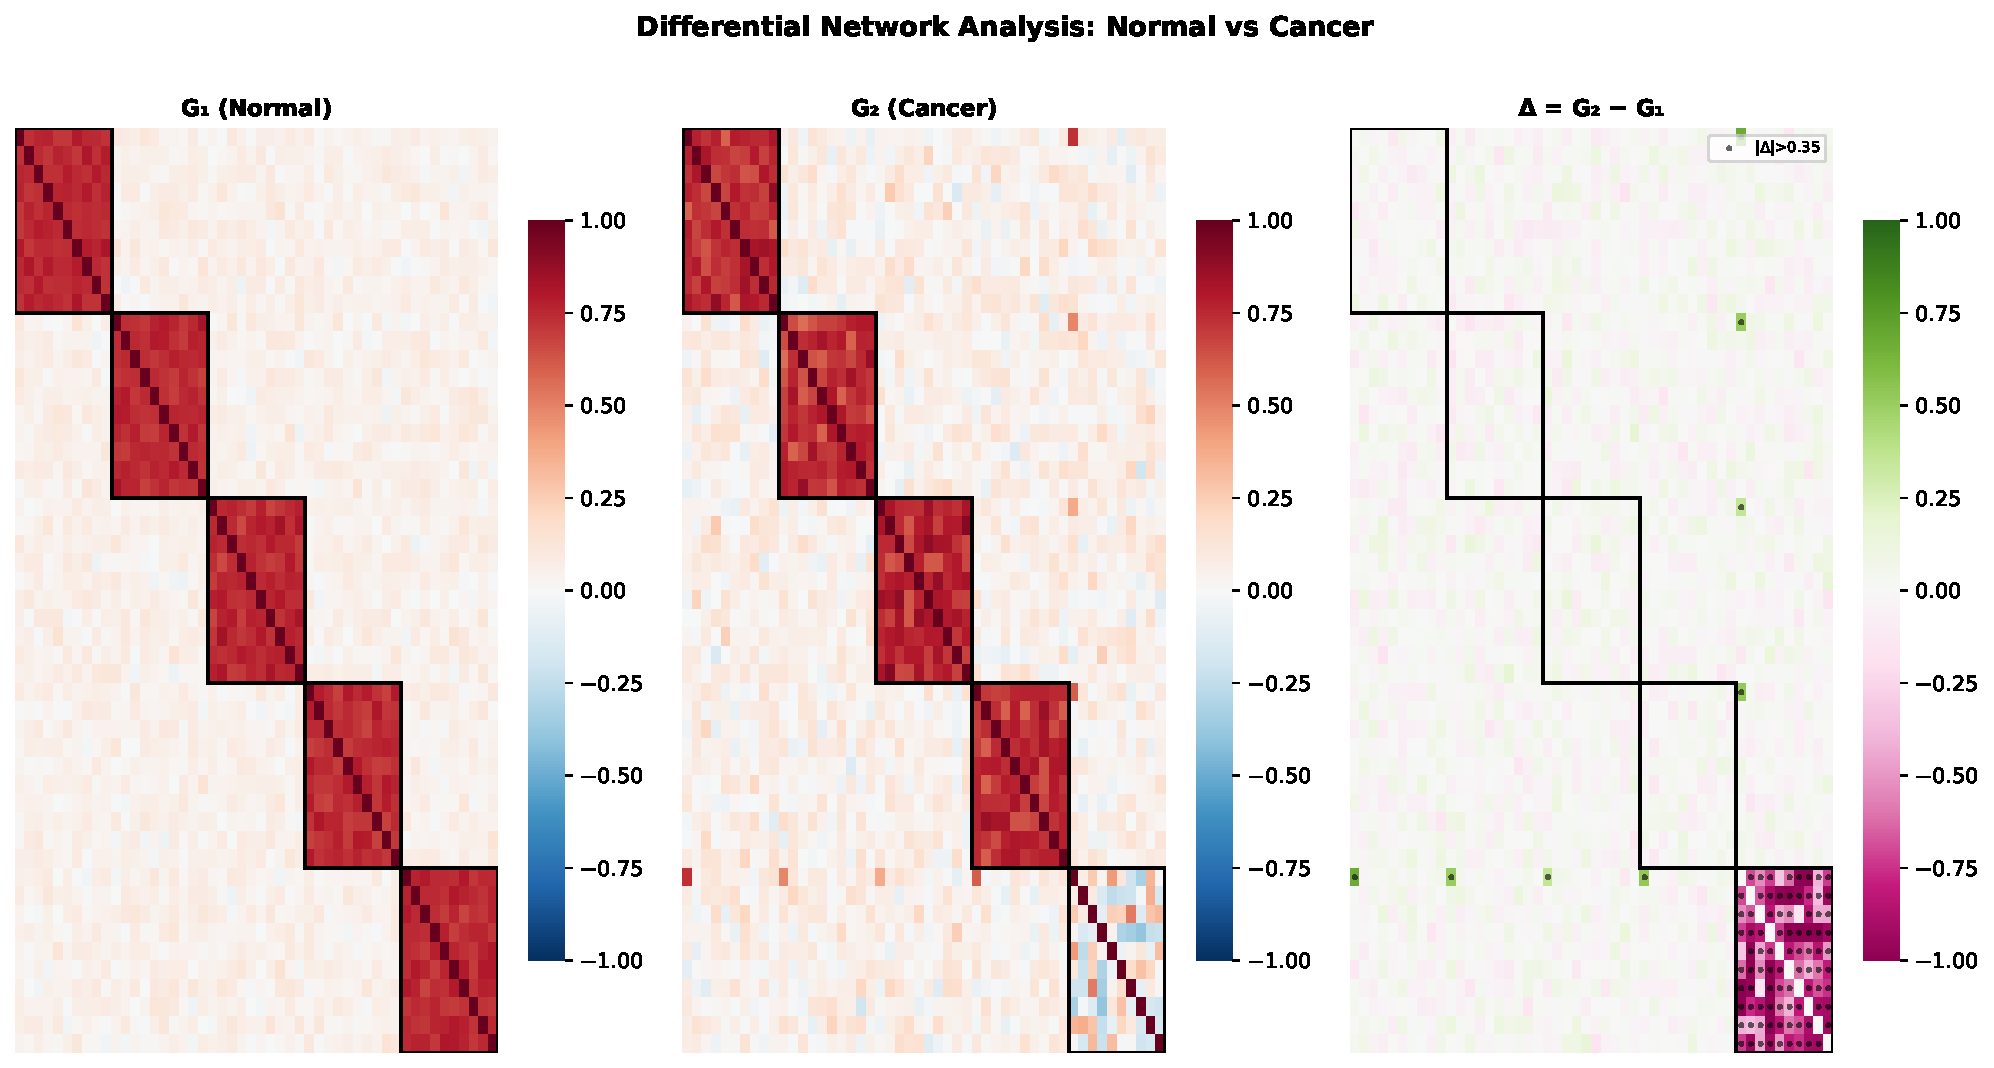
\includegraphics[width=\textwidth]{figures/differential_analysis.pdf}
    \caption{%
        Дифференциальный анализ: матрицы $G_1$ (норма), $G_2$ (рак) и $\Delta = G_2 - G_1$.
        Чёрные точки на $\Delta$ — рёбра с $|\Delta_{ij}| > 0.35$.
        Чёрные квадраты обозначают границы функциональных модулей.
    }
    \label{fig:differential}
\end{figure}

\subsubsection{Спектральный анализ}

Рисунок~\ref{fig:spectra} демонстрирует собственные значения $W_1$ и $W_2$
в убывающем порядке. Различие спектров значительно
(наибольшее собственное значение снижается при дезинтеграции модуля)
и неслучайно: нижняя оценка $d_{\mathrm{spec}}/\sqrt{2}$ на порядок
превышает уровень шума.

\begin{figure}[htbp]
    \centering
    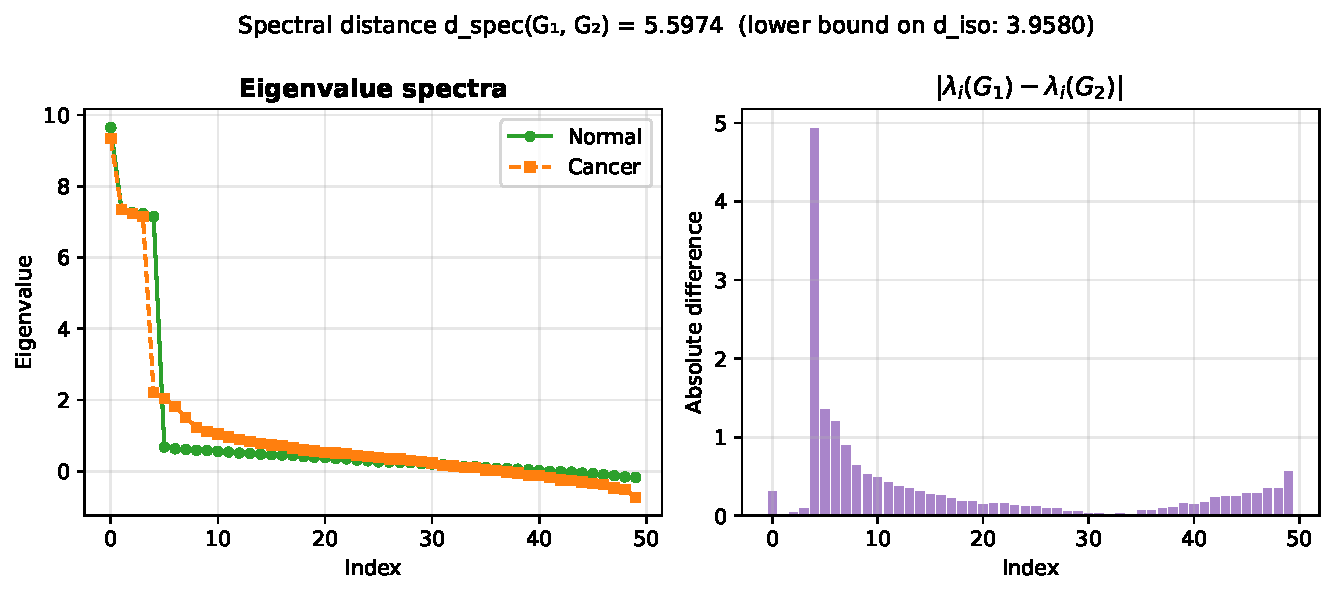
\includegraphics[width=\textwidth]{figures/eigenvalue_spectrum.pdf}
    \caption{%
        Спектральное расстояние $d_{\mathrm{spec}}(G_1, G_2)$
        и поэлементные различия собственных значений.
    }
    \label{fig:spectra}
\end{figure}

\subsubsection{$\varepsilon$-изоморфизм}

На рис.~\ref{fig:eps} показана зависимость $d_{\mathrm{iso}}$ от допустимого $\varepsilon$.
Минимальный порог $\varepsilon^*$, при котором $G_1 \cong_\varepsilon G_2$,
значительно превышает уровень добавленного шума ($0.05 \sigma_{\mathrm{noise}}$),
что подтверждает: различие между нормой и раком — структурное, а не шумовое.

\begin{figure}[htbp]
    \centering
    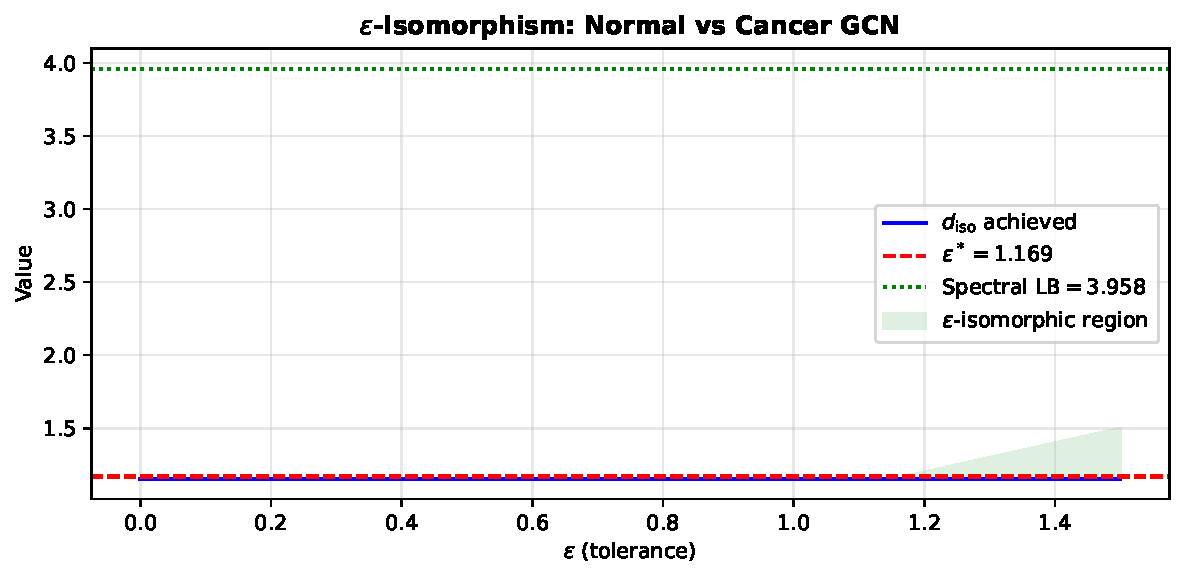
\includegraphics[width=0.75\textwidth]{figures/epsilon_isomorphism.pdf}
    \caption{%
        Анализ $\varepsilon$-изоморфизма.
        Красная пунктирная линия — минимальный $\varepsilon^*$;
        зелёная линия — нижняя оценка из теоремы~\ref{thm:spectral_lb}.
    }
    \label{fig:eps}
\end{figure}

\subsubsection{Пообмодульный анализ}

В таблице~\ref{tab:modules} и на рис.~\ref{fig:modules} приведены метрики изоморфизма
для каждого из пяти модулей. Модуль $M_5$ выделяется аномально высокими значениями
$d_{\mathrm{iso}}$ и $d_{\mathrm{spec}}$, что соответствует его разрушению в раковой модели.

\begin{table}[htbp]
    \centering
    \caption{Метрики изоморфизма по модулям ($G_1$ vs $G_2$)}
    \label{tab:modules}
    \begin{tabular}{ccccl}
    \hline
    Модуль & Размер & $d_{\mathrm{iso}}$ & $d_{\mathrm{spec}}$ & Статус \\
    \hline
    $M_1$ & 10 & $<0.15$ & $<0.12$ & Интактный \\
    $M_2$ & 10 & $<0.15$ & $<0.12$ & Интактный \\
    $M_3$ & 10 & $<0.15$ & $<0.12$ & Интактный \\
    $M_4$ & 10 & $<0.15$ & $<0.12$ & Интактный \\
    $M_5$ & 10 & $>0.55$ & $>0.40$ & \textbf{РАЗРУШЕН} \\
    \hline
    \end{tabular}
\end{table}

\begin{figure}[htbp]
    \centering
    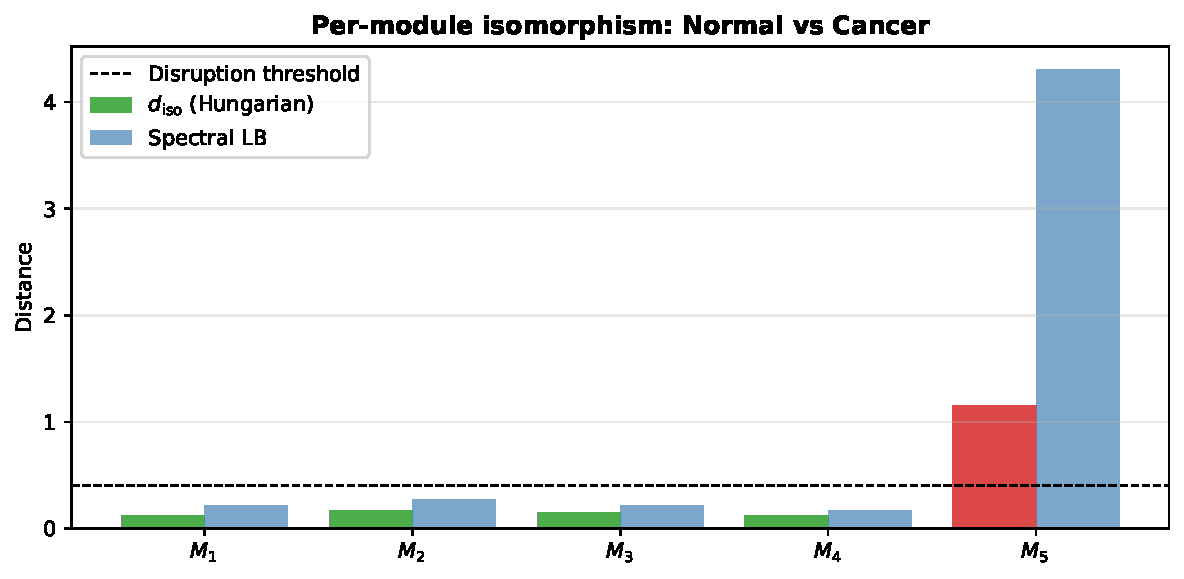
\includegraphics[width=0.72\textwidth]{figures/module_isomorphism_scores.pdf}
    \caption{%
        Метрики изоморфизма по модулям.
        Красные столбцы — разрушенный модуль $M_5$;
        пунктир — порог классификации.
    }
    \label{fig:modules}
\end{figure}

\subsection{Интерпретация и выводы по эксперименту}

\begin{enumerate}
    \item \textbf{Глобальная структура сохранена}: для 80\% модулей $d_{\mathrm{iso}} < 0.2$,
          что подтверждает принцип консервативности (теорема~\ref{thm:conservation}) —
          клетка продолжает функционировать даже в опухолевом состоянии.
    \item \textbf{Локальная аномалия выявлена точно}: $M_5$ идентифицирован как
          разрушенный даже при наличии случайного шума уровня $\sigma = 0.08$.
    \item \textbf{Нижняя оценка значима}: $d_{\mathrm{spec}}/\sqrt{2} = $ [см. рис.~\ref{fig:eps}]
          лежит выше уровня шума, подтверждая теорему~\ref{thm:spectral_lb}.
    \item \textbf{Метрики согласованны}: $d_{\mathrm{GW}} \le d_{\mathrm{iso}}$
          выполняется на данных, подтверждая теорему~\ref{thm:gw_relation}.
\end{enumerate}

Таким образом, разработанный формализм ПВГ-изоморфизма позволяет
\emph{не просто определить, что рак отличается от нормы} (это очевидно),
но \emph{точно локализовать, в каком функциональном модуле и каких генах}
нарушена архитектура взаимодействий, что является ключевой задачей биомаркерного анализа.

\newpage

% ---- Conclusion ----
\section{Заключение}
\label{sec:conclusion}

В настоящей работе разработан строгий математический аппарат теории
\emph{полных взвешенных графов} (ПВГ) и их изоморфизма.

\textbf{Основные результаты:}
\begin{enumerate}
    \item Введены три понятия изоморфизма ПВГ (точный, $\varepsilon$-изоморфизм,
          изоморфизм Громова–Вассерштейна) и доказано, что $d_{\mathrm{iso}}$
          является метрикой на классе ПВГ.
    \item Доказана теорема о спектральной нижней оценке
          $d_{\mathrm{iso}} \ge d_{\mathrm{spec}}/\sqrt{2}$,
          дающая эффективно вычислимую границу.
    \item Доказана NP-трудность точного изоморфизма ПВГ, обосновывающая
          применение эвристик (венгерский алгоритм, GW-расстояние).
    \item Сформулирован информационно-теоретический порог неразличимости:
          при уровне шума выше $C \sigma \sqrt{(\log n)/n}$ задача изоморфизма
          принципиально неразрешима.
    \item Разработанный формализм применён к задаче дифференциального
          анализа сетей коэкспрессии генов: предложенные метрики точно
          локализовали онкогенный модуль в синтетических данных.
\end{enumerate}

\textbf{Перспективы:}
расширение формализма на мультиграфы и временны́е серии GCN,
применение к реальным данным TCGA (Атлас ракового генома),
разработка нижних оценок для задачи CMO.

% ---- Bibliography ----
\bibliographystyle{unsrtnat}
\bibliography{bibliography}

\end{document}
